\documentclass{standalone}
\usepackage{graphicx}	
\usepackage{amssymb, amsmath}
\usepackage{color}

\usepackage{tikz}
\usetikzlibrary{intersections, backgrounds}
\usepackage{pgfmath}

\definecolor{light}{RGB}{220, 188, 188}
\definecolor{mid}{RGB}{185, 124, 124}
\definecolor{dark}{RGB}{143, 39, 39}
\definecolor{highlight}{RGB}{180, 31, 180}
\definecolor{gray10}{gray}{0.1}
\definecolor{gray20}{gray}{0.2}
\definecolor{gray30}{gray}{0.3}
\definecolor{gray40}{gray}{0.4}
\definecolor{gray60}{gray}{0.6}
\definecolor{gray70}{gray}{0.7}
\definecolor{gray80}{gray}{0.8}
\definecolor{gray90}{gray}{0.9}
\definecolor{gray95}{gray}{0.95}

\begin{document}

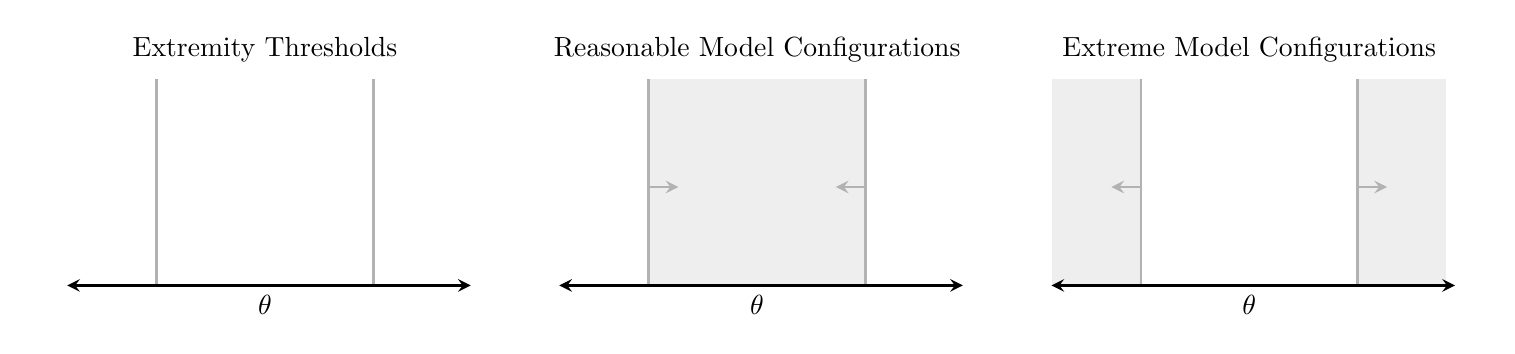
\begin{tikzpicture}[scale=0.25, thick]

  \begin{scope}[shift={(0, 0)}]
    \draw[white] (-12, -2) rectangle (12, 13);
    
    \node at (0, 12) { Extremity Thresholds };
  
    \draw[-, color=gray70, line width=1] (-5.5, 0) -- (-5.5, 10.5);
  
    \draw[-, color=gray70, line width=1] (5.5, 0) -- (5.5, 10.5);
  
    \draw [<->, >=stealth, line width=1] (-10.05, 0) -- +(20.5, 0);
    \node at (0, -1) { $\theta$ };
  \end{scope}
  
  \begin{scope}[shift={(25, 0)}]
    \draw[white] (-12, -2) rectangle (12, 13);
    
    \node at (0, 12) { Reasonable Model Configurations };
  
    \fill[color=gray80, opacity=0.33] (-5.5, 0) rectangle (5.5, 10.5);
    
    \draw[-, color=gray70, line width=1] (-5.5, 0) -- (-5.5, 10.5);
    \draw[->, >=stealth, line width=1, color=gray70] (-5.5, 5) -- +(1.5, 0);
  
    \draw[-, color=gray70, line width=1] (5.5, 0) -- (5.5, 10.5);
    \draw[->, >=stealth, line width=1, color=gray70] (5.5, 5) -- +(-1.5, 0);
  
    \draw [<->, >=stealth, line width=1] (-10.05, 0) -- +(20.5, 0);
    \node[] at (0, -1) { $\theta$ };
  \end{scope}
  
  \begin{scope}[shift={(50, 0)}]
    \draw[white] (-12, -2) rectangle (12, 13);
    
    \node at (0, 12) { Extreme Model Configurations };
  
    \fill[color=gray80, opacity=0.33] (-10, 0) rectangle (-5.5, 10.5);
    \draw[-, color=gray70, line width=1] (-5.5, 0) -- (-5.5, 10.5);
    \draw[->, >=stealth, line width=1, color=gray70] (-5.5, 5) -- +(-1.5, 0);
  
    \fill[color=gray80, opacity=0.33] (10, 0) rectangle (5.5, 10.5);
    \draw[-, color=gray70, line width=1] (5.5, 0) -- (5.5, 10.5);
    \draw[->, >=stealth, line width=1, color=gray70] (5.5, 5) -- +(1.5, 0);
  
    \draw [<->, >=stealth, line width=1] (-10.05, 0) -- +(20.5, 0);
    \node[] at (0, -1) { $\theta$ };
  \end{scope}
  
\end{tikzpicture}

\end{document}  